% Enterprise software enable multiparty conference scenarios within a guarded enterprise network. Usually with a session-centric client-server architecture. Enterprise communication software usually uses an \gls{sbc} to communicate with the outside world. \gls{wrtc} is not designed to work with current \gls{sbc} deployments. We look into how we can adapt an enterprise firewall to work with \gls{wrtc}.

In this section I will start by pointing out the differences between the gateway used for testing purposes and the gateway that would have to be implemented for VA. Starting with the traffic proxy and media server. Then I will describe the differences in the signaling. Lastly I will introduce the problems of crossing the enterprise firewall.

\section{The traffic proxy and media server}
The media in VA travels over raw RTP streams. The traffic proxy needs to handle ICE and the translation between RTP and SRTP-DTLS like in the previous chapter, but in addition it needs to do multiplexing and demultiplexing of the streams.

\section{Signaling}
Since the signaling is proprietary in VA, it would have to be upgraded to support the \gls{sdp} used in the \gls{rtcweb} standard, or we could develop a way of manipulating the \gls{sdp} in the signaling proxy. However, we can still use the same protocols for transmitting the signaling, but we have to use a gateway to allow the messages to travel over HTTP as well. This could be accomplished using JSON over WebSockets as an example.

\section{The enterprise firewall}
Enterprises such as Visual Solutions use firewalls to enforce Internet Protocol access policies at the edge of their networks. These policies relate to who is allowed to access which resources. The firewall are often implemented using 5-tuple rules (source and destination IP address, source and destination ports, and transport protocol). Typically firewalls were developed to handle client-server protocols such as web browsing, email, and file transfer\cite{johnston_taking_2013}. Peer-to-peer communication systems are bigger challenges to firewalls, and since \gls{wrtc} is designed to work peer-to-peer, this introduces some problems. \gls{rtp} packets are typically described as peer-to-peer flows. Media can be sent from inside the firewall, but the reverse flow often gets blocked. This is why \gls{ice} was developed, to make firewall traversal easier. But enterprise communication software usually has a client-server architecture, to communicate with entities outside the enterprise network, it is common to use a \gls{sbc}. Currently \gls{sbc}s won't work well with \gls{wrtc}. This raises some questions:

\begin{itemize}
\item{How can the enterprise firewall adapt to \gls{wrtc}?}
\item{How can the enterprise firewall detect and apply policy to \gls{wrtc} flows?}
\end{itemize}

\section{Session Border Controllers}

\begin{figure}[here]
\centerline{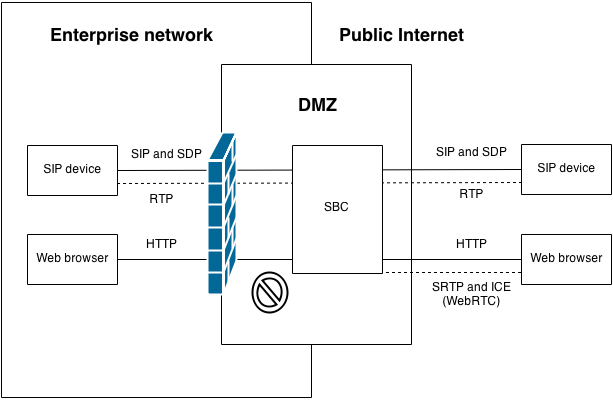
\includegraphics[scale=0.5]{sbcpolicy.png}}
\caption{The SBC opens firewall to allow for enterprise communication, but WebRTC traffic uses HTTP which is not intercepted, and the media path is blocked.}
\label{fig:sbc-policy}
\end{figure}

An \gls{sbc} is essentially an application layer firewall with a signaling and media application layer gateway built in. The \gls{sbc} is usually connected in an enterprise demilitarized zone(DMZ) as a trusted enterprise network element. It blocks all unauthorized signaling and media flows, and provides a point of policy enforcement as shown in Figure \ref{fig:sbc-policy}. As specified by IETF\cite{sbc} a \gls{sbc} should support \gls{sip}, \gls{rtp}, and \gls{srtp}. \gls{sip} is a signaling protocol used for \gls{voip} and video communications to establish \gls{rtp} media sessions. By parsing \gls{sip} messages, the \gls{sbc} is able to discover the transport addresses (5-tuple) to be used for the media session. The \gls{sbc} opens a filter rule permitting the \gls{rtp} traffic, and the \gls{rtp} media session is able to traverse the firewall. Since \gls{sbc}s are widely deployed it makes sense to reuse them for \gls{wrtc}. However, there are problems with this approach. \gls{wrtc} has no concept of sessions; instead, it has a concept of `streams'. Streams have media sources and sinks that generate and consume media flows. One possible apporach would be to translate every \gls{wrtc} session that crosses enterprise boundaries into a communication session that its existing infrastructure could handle in a session-centric manner. This could mean converting a \gls{wrtc} session into a SIP session, then converting back again.

The \gls{sbc} should either be upgraded to support \gls{wrtc} or we should opt for another way of detecting \gls{wrtc} flows.

\section{WebRTC firewall traversal}
If upgrading the \gls{sbc} is not trivial, we can look at the other planes for detecting an incoming \gls{wrtc} session:

\subsection{ICE}
There is a standard type of signaling protocol used for establishing media flows as part of \gls{wrtc}. It is built into the \gls{ice} protocol used for traversing firewalls. Before any media flows, \gls{ice} is run between two browsers. This could be used to detect an \gls{ice} exchange starting up across the enterprise border. This could then be used to distinguish a \gls{wrtc} media flow across the border, allowing policy to be applied.

\subsection{SRTP}
Another approach might be to use SRTP key negotiation along with \gls{dtls} to authenticate the media flow. For example, since SRTP-DTLS is used for key management, the secure edge could act as a man-in-the-middle an hence validate the public key in the fingerprint. A self-signed key from the browser could be stored in an enterprise key server. This could allow the secure edge to authenticate the browser inside the enterprise network and apply appropriate policy.

\subsection{Media relay}
Another approach would be to require a media relay to be used for \gls{wrtc} media sessions crossing the enterprise boundary. There is a standard protocol for this relay, known as \gls{turn}. The enterprise firewall would be configured to block non-relayed \gls{wrtc} media flows. The enterprise would then deploy a \gls{turn} server in the \gls{dmz}, and permit media flows that go through this server. During media flow setup, the TURN server could authenticate the user and also learn what type of media flow is to be set up based on the bandwidth requested. Policy could then be applied to this media flow.

\section{Summary}
Doing peer-to-peer communication crossing enterprise networks are difficult. It might not be trivial to upgrade current SBC implementations, therefore I looked into other ways of detecting \gls{wrtc} traffic for applying policy to the media flows. The next chapter will look at some of the challenges of creating a mobile \gls{wrtc} client.